\chapter{Background Theory of Bayesian Techniques and WEST Interferometry}

This chapter aims to equip the reader with the necessary background theory required to reproduce this work and to understand the origin of the inferred electron density profiles presented in the results. It first describes a tokamak fusion device and some relevant physics concepts behind its function. It then describes in a high level manner the inference carried out by Blaise Faugeras and team with their code known as \gls{nice} \cite{nice}. After, the chapter outlines Bayesian inference and how a specific implimentation can be used to solve a simple regression problem. Interferometry is introduced in enough detail to understand how the electron density profile could be infered from its data. The Bayesian inference method introduced for the simple regression problem is then altered to allow this inference. Various options for advanced alterations are also explained here and explored in the results section.

\section{The Tokamak}

\begin{figure}[H]
  \centering
  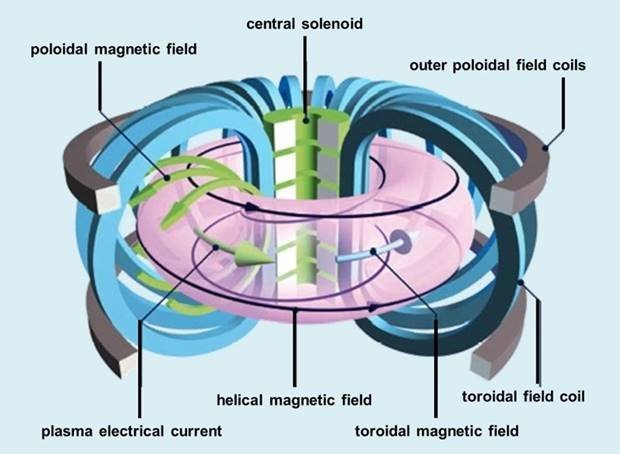
\includegraphics[width=10cm]{images/tokamak.jpg}
  \caption{A tokamak and relevant magnetic fields that create the helical particle trajectory \cite{tokamakSchema}.}
  \label{fig:tokamakSchema}
\end{figure}

Tokamak is a class of fusion devices whose name comes from the abbreviation of a Russian phrase which means ``toroidal chamber with magnetic coils''. It consists of a doughnut shaped vacuum chamber surrounded by powerful magnets that aim to confine a high temperature plasma that would otherwise vaporise the chamber. The plasma pressure and temperature are fundamental parameters in the context of nuclear fusion because they dictate the conditions required to overcome the electrostatic repulsion between positively charged atomic nuclei and bring them close enough for the strong nuclear force to initiate fusion reactions. In the core of stars like our Sun, the immense pressure and temperature generated by the gravitational collapse create the conditions where hydrogen nuclei (protons) can overcome their natural repulsion and fuse into helium, releasing a tremendous amount of energy in the process. To initiate fusion, hydrogen must be heated to temperatures in the range of tens of millions of degrees Celsius. In a tokamak, this is mainly accomplished with ohmic heating via a driving plasma current and neutral gas injection. This involves accelerating hydrogen ions to high speeds with electric fields and neutralising them the instant before they enter the chamber. The resulting plasma attains the required temperature, allowing nuclei to collide with sufficient energy for fusion reactions to occur. Figure \ref{fig:tokamakSchema} shows the position of various magnetic field coils within the tokamak. The toroidal magnetic field exerts an inward force on the plasma thus raising its pressure. High pressure is required to increase the frequency of collisions so that the energy output can exceed the large heating energy input. The central solenoid induces a current in the plasma which produces the majority of the poloidal magnetic field. This field is essential for confinement but it also plays a key role in plasma stability. The outer poloidal field coils can be controlled in real time to help mitigate instabilities. A real time inference of the electron density profile would assist in identifying instabilities and informing the algorithm that drives the control coils to mitigate them. In addition to high temperature and pressure, the tokamak design seeks to maximize the confinement time of the plasma. This is essential to allow a sufficient number of fusion reactions to occur before the plasma cools down or loses its stability. The magnetic fields in a tokamak are carefully optimized to prevent rapid plasma loss and minimize heat loss through various mechanisms, including turbulent transport. The shape of the density profile has a large effect on the confinement time.

The combination of the toroidal and poloidal fields shown in figure \ref{fig:tokamakSchema} creates a helical magnetic field within the plasma. Electrons and ions are accelerated in opposite toroidal directions by the central solenoid yet both follow a trajectory along the magnetic field lines. This is because a charged particle moving across a magnetic field succumbs to a force perpendicular to its motion. This causes them to gyrate around the magnetic field lines and confines them to follow the magnetic field lines. This is an oversimplification and in reality there are drift forces that cause the particles the deviate from following the magnetic field lines exactly. Collisions also cause deviations. A detailed description of particle motion within a magnetic field is not needed for this thesis. It is enough to know that the particles in general follow the helical path of the magnetic field lines with a small gyration around the field line. In many models used for data analysis the assumption that particles follow the magnetic field lines is used, including within this thesis. 

The magnetic field lines are confined to magnetic flux surfaces, figure \ref{fig:magfluxsurf}. The toroidal and poloidal flux is constant on magnetic flux surfaces, there is 0 flux across magnetic flux surfaces. Since we assume that the particles follow the magnetic field lines which are strictly bound to these surfaces, we also assume that the density is constant on these surfaces. This allows the density of the entire cross-section to be expressed with a 1D profile as a function of normalised radius $\rho$ for example, see \gls{nice}'s profile, figure \ref{fig:nice_example}. Where $\rho$ is 0 at the magnetic axis and 1 at the plasma boundary. The magnetic axis is very center point of the core and defined as where the poloidal magnetic flux is minimum and the plasma boundary is the last closed flux surface. Particles past the plasma boundary are no longer bound and may interact with the plasma wall. The existence of nested magnetic flux surfaces shown in figure \ref{fig:magfluxsurf} rely on the ideal \gls{mhd} assumptions. Experiments frequently discover magnetic islands which discredits the assumption of nested flux surfaces. The electron density profiles inferred by \gls{nice} and this work make the nested flux surface assumption, although for many applications such as real time control, a highly accurate inference is often not required.

\begin{figure}
  \centering
  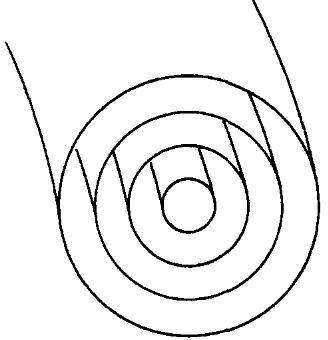
\includegraphics[width=5cm]{images/fluxsurf.png}
  \caption{Magnetic flux surfaces \cite{wessontokamak}.}
  \label{fig:magfluxsurf}
\end{figure}

\section{NICE}

\gls{nice} is an equilibrium reconstruction code that is routinley deployed for the \gls{west} tokamak. It is relevant because it computes an inference of the electron density profile that is available for comparison to the profile inferred in this work, although \glspl{nice} main objective is to infer the shape and position of the magnetic flux surfaces. \gls{nice} uses magnetic diagnostics. At \gls{west} these include 421 pickup coils, 36 flux loops and 12 Rogowski coils \cite{westmagdiag}. Magnetic diagnostics provide the majority of the information. \gls{nice} also uses interferometry, polarimetry, motional stark effect and pressure measurements. Equation \ref{eq:int_phase} and \ref{eq:pol_farad} further in the chapter, show how interferometry and polarimetry together can provide information about the poloidal magnetic field, which directly affects the magnetic flux and thus magnetic flux surfaces. \gls{nice} performs the inference by minimising a cost function. The cost function determines how well a physical state of the system matches the data received. A state is a specific position and shape of the magnetic flux surfaces and electron density profile. This requires a forward model. The forward model takes a state of the system and attempts to compute the signals that would be received by error free diagnostics if that state was the ground truth. The forward model is a simplified mathematical representation of the measurement process and can never be 100\% accurate. This introduces errors in the inference that need to be accounted for. The signals from the forward model can be compared to the actual signals received by the diagnostics to compute the cost function. By minimising the cost function the state that best matches the data is found. \gls{nice} uses \gls{sqp} as the minimisation algorithm. The optimal state of the system is then stored in the \gls{imas} database for \gls{west}. This includes the 1D electron density profile used as a comparison for the profile inferred in this work. \gls{nice} also imposes regularisation terms on their cost function. These penalise the cost function when state properties have features that disagree with prior knowledge. This includes smoothness. We expect the magnetic flux surfaces and electron density profile, to be continuous and smooth. A state inputted into the cost function that is not smooth triggers the regularisation term which causes the cost function to be larger. Minimising the cost function now also leads to smooth magnetic flux surfaces and electron density profile. This leads to a difficult question, how smooth should it be? They also have a regularisation term to penalise the cost function if the electron density profile is far from 0 at the last closed flux surface or plasma boundary. It is prior knowledge that the electron density is near 0 at the plasma boundary. How close to 0, and how strong should the regularisation be is still an open question. This work's approach has direct analogues to these regularisation terms. As explained later in more detail the length scale controls smoothness and an artificial observation ensures the density is close to zero at the plasma boundary. Figure \ref{fig:nice_example} shows an example of a \gls{nice} inferred electron density profile. It is modelled with a cubic spline function. It is the parameters of the cubic spline that are inputted into the cost function. The errors are calculated using a sensitivity method. In short, the error is deemed larger for the electron density of a particular normalised radius if a large change in the density leads to a small change in the cost function. In this case, we cannot be certain what density is better because many lead to a similarly low cost function and thus match the data similarly well. To include some more details, the \gls{sqp} minimisation algorithm computes the hessian of the cost function for minimisation, but this hessian can also be used to measure the sensitivity and thus the errors. The diagonal of the hessian contains the second differential of the cost function for each input parameter. This describes the curvature of the cost function in the direction of each parameter. A smaller curvature means a smaller sensitivity and thus a larger error.

\begin{figure}
  \centering
  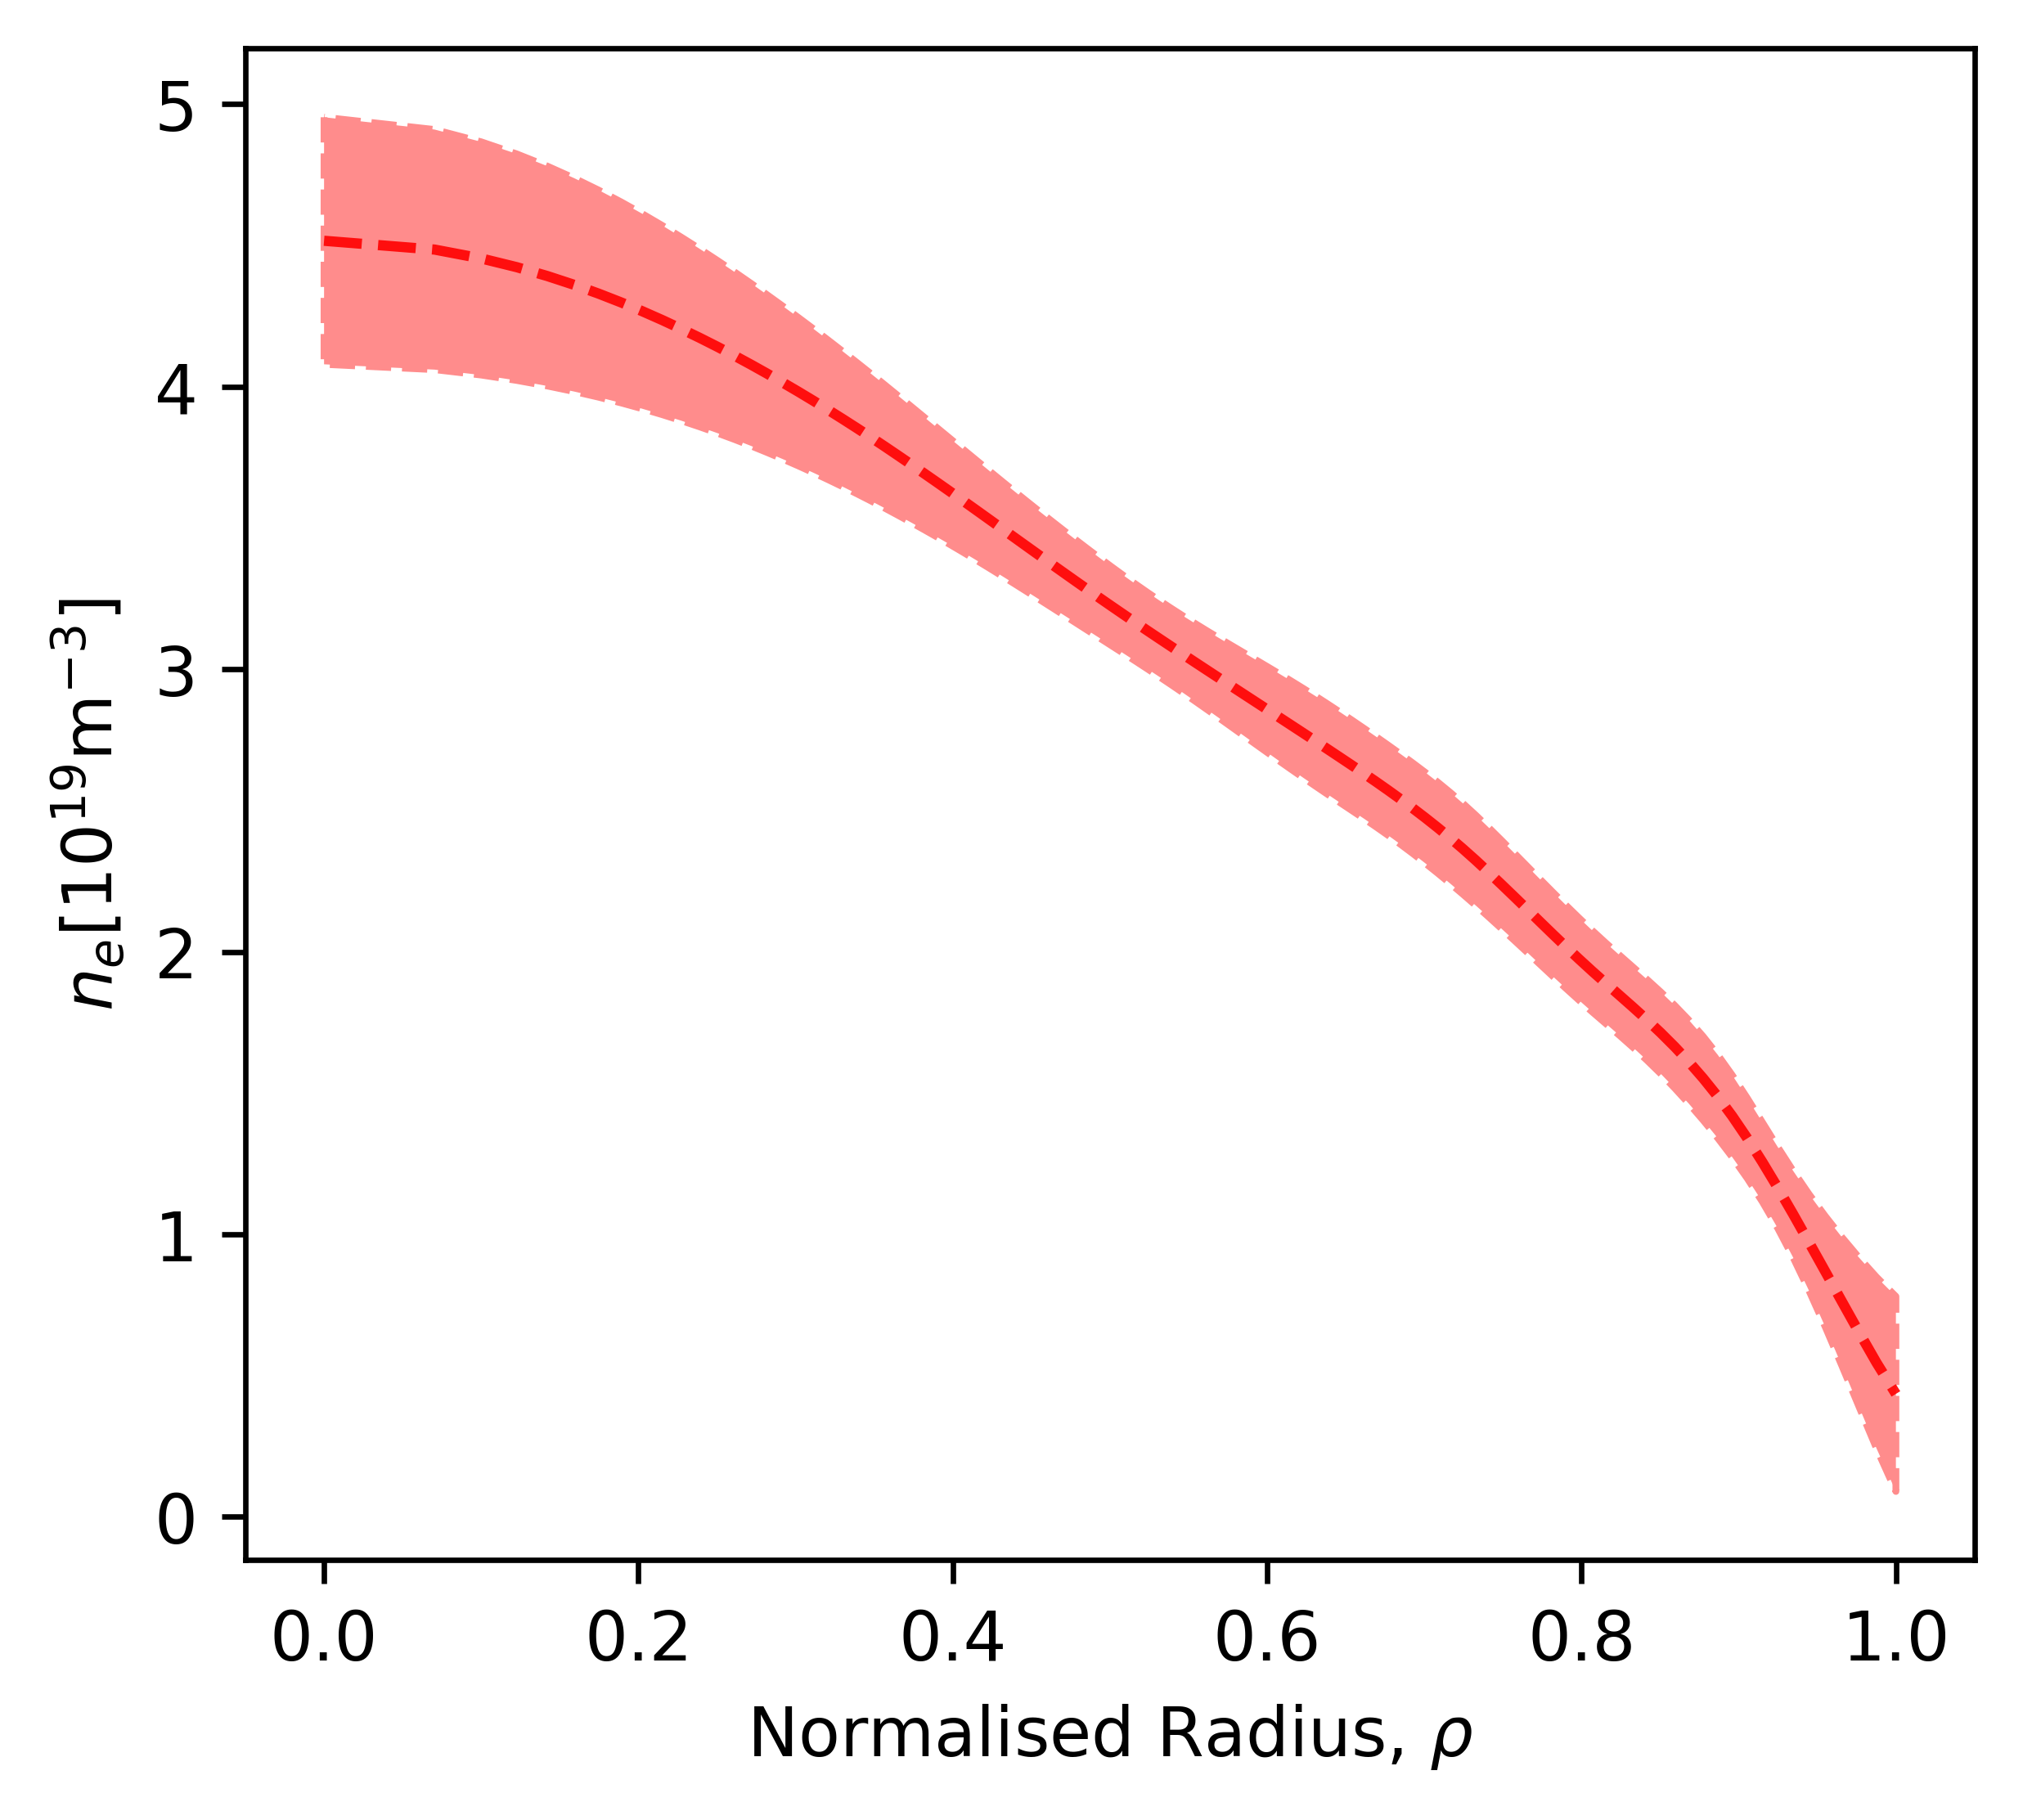
\includegraphics[width=13cm]{images/niceExample.png}
  \caption{Electron density profile inferred by NICE for an instance in time within the WEST tokamak.}
  \label{fig:nice_example}
\end{figure}

\section{Bayesian Inference and the Simple Regression Problem}
\label{sec:BIandSRP}

This work aims to use Bayesian inference to obtain the electron density profile. Bayesian inference will be introduced generally and then it will be used to define a specific implemtation applied to a simple regression problem. The method introduced will later be extended to solve the problem of infering the electron density profile with interferometry data. Bayes' theorem for a physical quantity of interest $q$ is expressed as,

\begin{equation}
P(q|D,I) = \frac{P(D|q,I) P(q|I)}{P(D|I)},
\label{eq:bayesth}
\end{equation}

\noindent the posterior $P(q|D,I)$ is the probability density distribution of $q$ given the measured data $D$ and some prior information $I$. The $q$ that maxemises the posterior is the most probable value of $q$ given the data and prior information. The uncertainty of $q$ can also be obtained from the posterior. The likelihood $P(D|q,I)$ is the probability density function that expresses the probability of the measured data given a fixed value of $q$ and the prior information. The likelihood is described by the experimental error for the data collection. The prior $P(q|I)$ contains information assumed about $q$ before the data is taken. The marginal likelihood or evidence $P(D|I)$ is simply the probability of the data given the prior information only. For posterior computation, the marginal likelihood serves as a normalisation factor. Normalisation is often carried out with other means to simplify the posterior computation. Although the marginal likelihood can be used to tune hyperparameters. For example, the degree or strength of prior information is uncertain and by finding the strength that maximises the marginal likelihood we find the prior that matches the data the best. Maximising the marginal likelihood to tune the hyperparameters also aids in avoiding over-fitting, as the trade off between model complexity and data-fit is automatic via Occam's razor principle \cite{oscraz}. The marginal likelihood method is powerful although it is important to remember that it is not perfect and does not guarantee to find the hyperparameters that lead to the most accurate posterior.

The version of Bayes' theorem for a simple regression problem is,

\begin{equation} 
  P(\vec{y}|\vec{d},\vec \epsilon, \theta) = \frac{P(\vec{d}|\vec{y},\vec \epsilon) P(\vec y|\theta)}{P(\vec y|\vec \epsilon, \theta)},
  \label{eq:bayesth_simple_regression}
\end{equation}

\noindent where $\vec y$ contains the values of a curve at regular $x$ values. The goal is to find the most likely $\vec y$ given the data and prior information. $\vec d$ contains curve measurements at known $x$ values with some experimental errors $\vec \epsilon$. $\theta$ is a set of parameters related to the prior form, explained more later. The likelihood and prior are going to be clearly defined as mutivariate Gaussians giving a multivariate Gaussian posterior wich needs to somehow model the curve $\vec y$. Figure \ref{fig:mvg} illustrates how a multivariate gaussian can model a curve. The functional form of a multivariate Gaussian is,

\begin{equation}
  \mathcal{N}(\vec y, \vec{\mu}, \Sigma) = \frac{1}{\sqrt{(2\pi)^{\frac{n}{2}}|\Sigma|}} \exp \left[{{-\frac{1}{2}(\vec{y}-\vec{\mu})^T\Sigma^{-1}(\vec{y}-\vec{\mu})}}\right],
  \label{eq:mvg}
\end{equation}

\noindent the mean vector $\vec{\mu}$ holds the $y$ values of the curve at regular intervals along the $x$ axis. The diagonal of the covariance matrix holds the standard deviations of each Gaussian within the multivariate. These represent the errors of the curve. Figure \ref{fig:mvg} shows 10 Gaussians with each mean connected by a straight line. In practice many Gaussians are used in a small space so that even a linear interpolation appears as a smooth curve. In our simple regression problem 101 Gaussians are used, thus $\vec y$ has a length of 101. The posterior that models the most likely curve given the data and prior information can be expressed as,

\begin{figure}
  \centering
  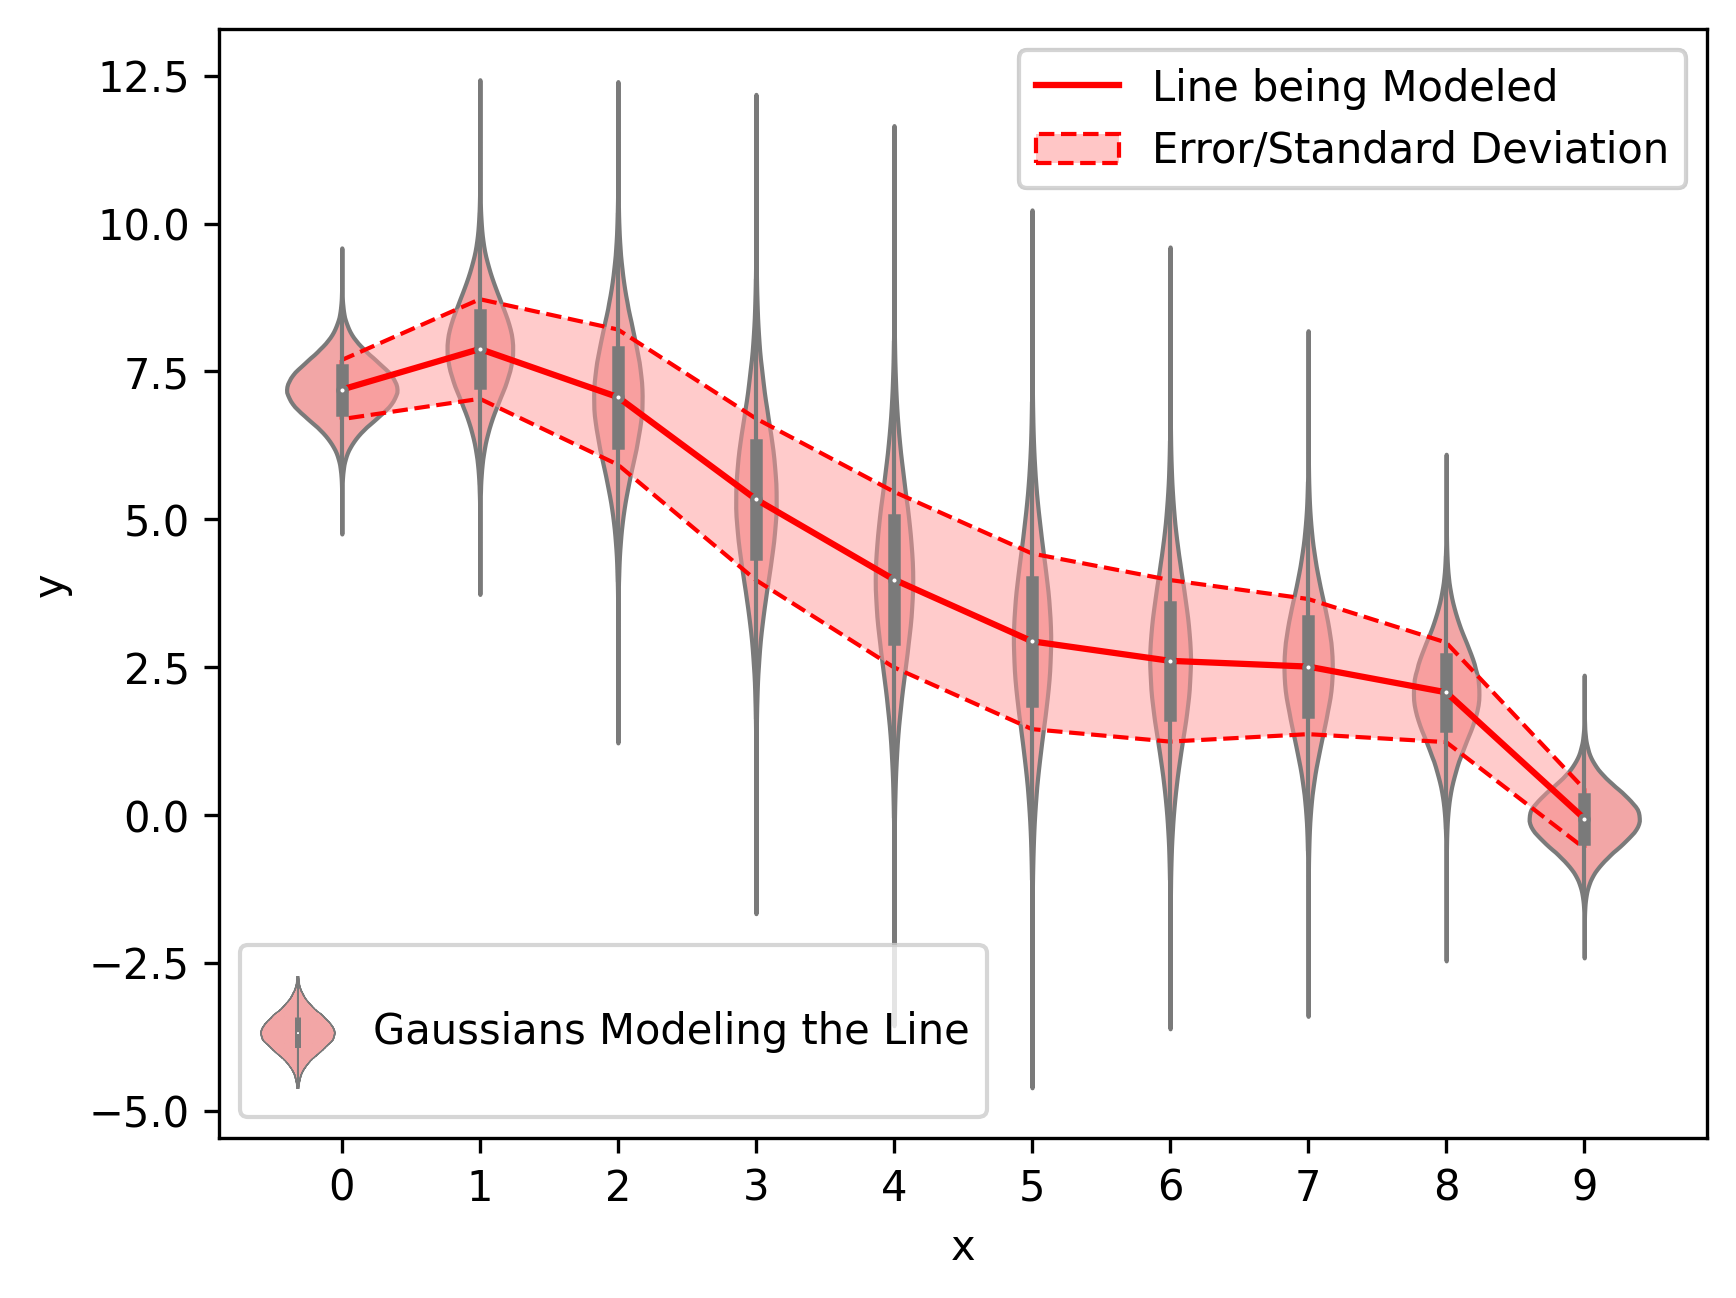
\includegraphics[width=10cm]{images/mvg.png}
  \caption{Illustrating how many Gaussians can model a curved line and its uncertainty.}
  \label{fig:mvg}
\end{figure}

\begin{equation}
  \mathcal{N}(\vec y, \vec{\mu}_{post}, \Sigma_{post}),
\end{equation}

\noindent where $\mu_{post}$ has a length of 101, the same as the unknown $y$ values.

In order to compute $\mu_{post}$ and $\Sigma{post}$ we must define the likelihood and prior. If $m$ measurements are taken the likelihood is defined as, 

\begin{equation}
  P(\vec{d}|\vec{y},\vec \epsilon) = \mathcal{N}(\vec{d}, \vec \mu_{li} = R\vec{y}, \Sigma_{li}),\, \Sigma_{li} = \vec{\epsilon}I = 
    \begin{bmatrix}
        \epsilon_1 & 0 & \hdots & 0\\
        0 & \epsilon_2 & \hdots & 0\\
        \vdots & \vdots & \ddots & 0 \\
        0 & 0 & 0 &\epsilon_m
    \end{bmatrix},
  \label{eq:likelihood}
\end{equation}

\noindent where $R$ is the responce matrix. Given some curve $\vec y$ to be true, $R \vec y$ is a vector that has the same length as $\vec d$ and contains the values of the curve $\vec y$ at the same $x$ values that the data was collected at. The responce matrix is an error free model of the measurement process. In the likelihood of figure \ref{fig:srpvis} the blue line is an example of a given $\vec{y}$ and if this was the ground truth and we took an error free measurement at the same $x$ points as our origional data then we would get the points indicated by the mean of each gaussian. These points are computed with $R\vec y$ and provide the mean vector of the likelihood. The likelihood represents the probability of getting the black data points given the blue line $\vec y$ is the ground truth. Regression is inherently an inverse problem and the responce matrix is a forward model. 

The prior is also a multi variate Gaussian and thus can be said to follow a gaussian process. Regression carried out with Bayesian inference and a Gaussian process prior is often reffered to as Gaussian Process Regression. Although, the method being introduced is more general than the typical implimentation of Gaussian Process Regression. This is so that it can easly be extended later to allow regression in situations where the data resides in a different space. To avoid confusion with the typical version of Gaussian Process Regression the term is not used for this implimentation. For an introduction to typical Gaussian Process Regression I suggest the text book Gaussain Processes for Machine Learning \cite{gp4ml}. The prior can be defined as,

\begin{equation}
  \mathcal{N}(\vec{y}, \vec \mu_{pr} = \vec{0}, K), \, K_{ij} = k(y_i, y_j) = \sigma^2 \exp\left[{\frac{(y_i - y_j)^2}{2l^2}}\right], 
  \label{eq:prior}
\end{equation}

\noindent where $\vec 0$ is a vector of 101 zeros, the same length as $\vec y$. The zero vector is a commonly used `non informative' prior mean vector. The covariance matrix $K$ is constructed using the kernel $k(x_i,x_j)$. The main role of the amplitude, $\sigma$, in the kernel is to set the prior strength. A high amplitude means the inference has a low prior strength and the resultant curve can be far from the prior mean $\mu_pr = \vec 0$. See the prior in figure \ref{fig:srpvis}, the amplitude $\sigma$ is the standard deviation of these gaussians shown. For visualisation purposes only 5 prior Gaussians are shown in figure \ref{fig:srpvis}, yet in reality there is 101, the same number as there are unknown $y$ values. The length scale, $l$ sets the strength of the correlation between the Gaussians. A low length scale means that only Gaussians close in $x$ are highly correlated. Gaussians further in $x$ would have a low correlation, meaning they can have a very different mean value. A low length scale allows the fitted curve to have more complexity similar to a high order polynomial and can lead to overfitting. A high length scale limits the fit's ability to curve sharply leading to a simple model, similar to a low order polynomial, leading to underfitting. A very high length scale leads to an almost linear fit. This prior is far from perfect. For instance, it is often known that the inferred values must be positive, for example, you cannot have a negative electron density. Since the prior mean vector is set to $\vec{0}$, a negative value is as likely to be inferred as a positive value. Since it is Gaussian, values close to 0 are more likely to be inferred than values far from 0. To mitigate this a high amplitude can be used to lower the prior strength and allow the data in the likelihood to have more influence on the posterior result. The kernel $k(x_i,x_j)$ in equation \ref{eq:prior} is known as the exponential square kernel. It is a very commonly used kernel but far from the only choice. The single value of the length scale prevents the inference from having long smooth regions with few features followed by regions of high variability. This can be an issue when inferring H-mode tokamak plasmas that have a sharp drop-off in density at the plasma edge. For these situations, a non-stationary kernel can be used that allows the length scale to be a function of $x$ which can then allow for posteriors of varying complexity. Regardless of the kernel used, deciding the optimal values of its parameters for a problem is not obvious. A common solution is to use the marginal likelihood of equation \ref{eq:bayesth}. The parameters that maximise the marginal likelihood also maximise the probability of the data being measured. The marginal likelihood method is also known for automatically deploying Occam's razor principle which finds a balance between closely fitting the data and having a simple model that accounts for the data's errors to have a more accurate inference \cite{oscraz} \cite{gp4ml}. Essentially maximising the marginal likelihood avoids overfitting. The maxemisation can be done with gradient based methods. Although this method is powerful it does not guarantee to produce parameters that lead to the most accurate fit. To get a more accurate fit, Bayesian sampling techniques can be used, although this is more computationally expensive.

\begin{figure}[H]
  \centering
  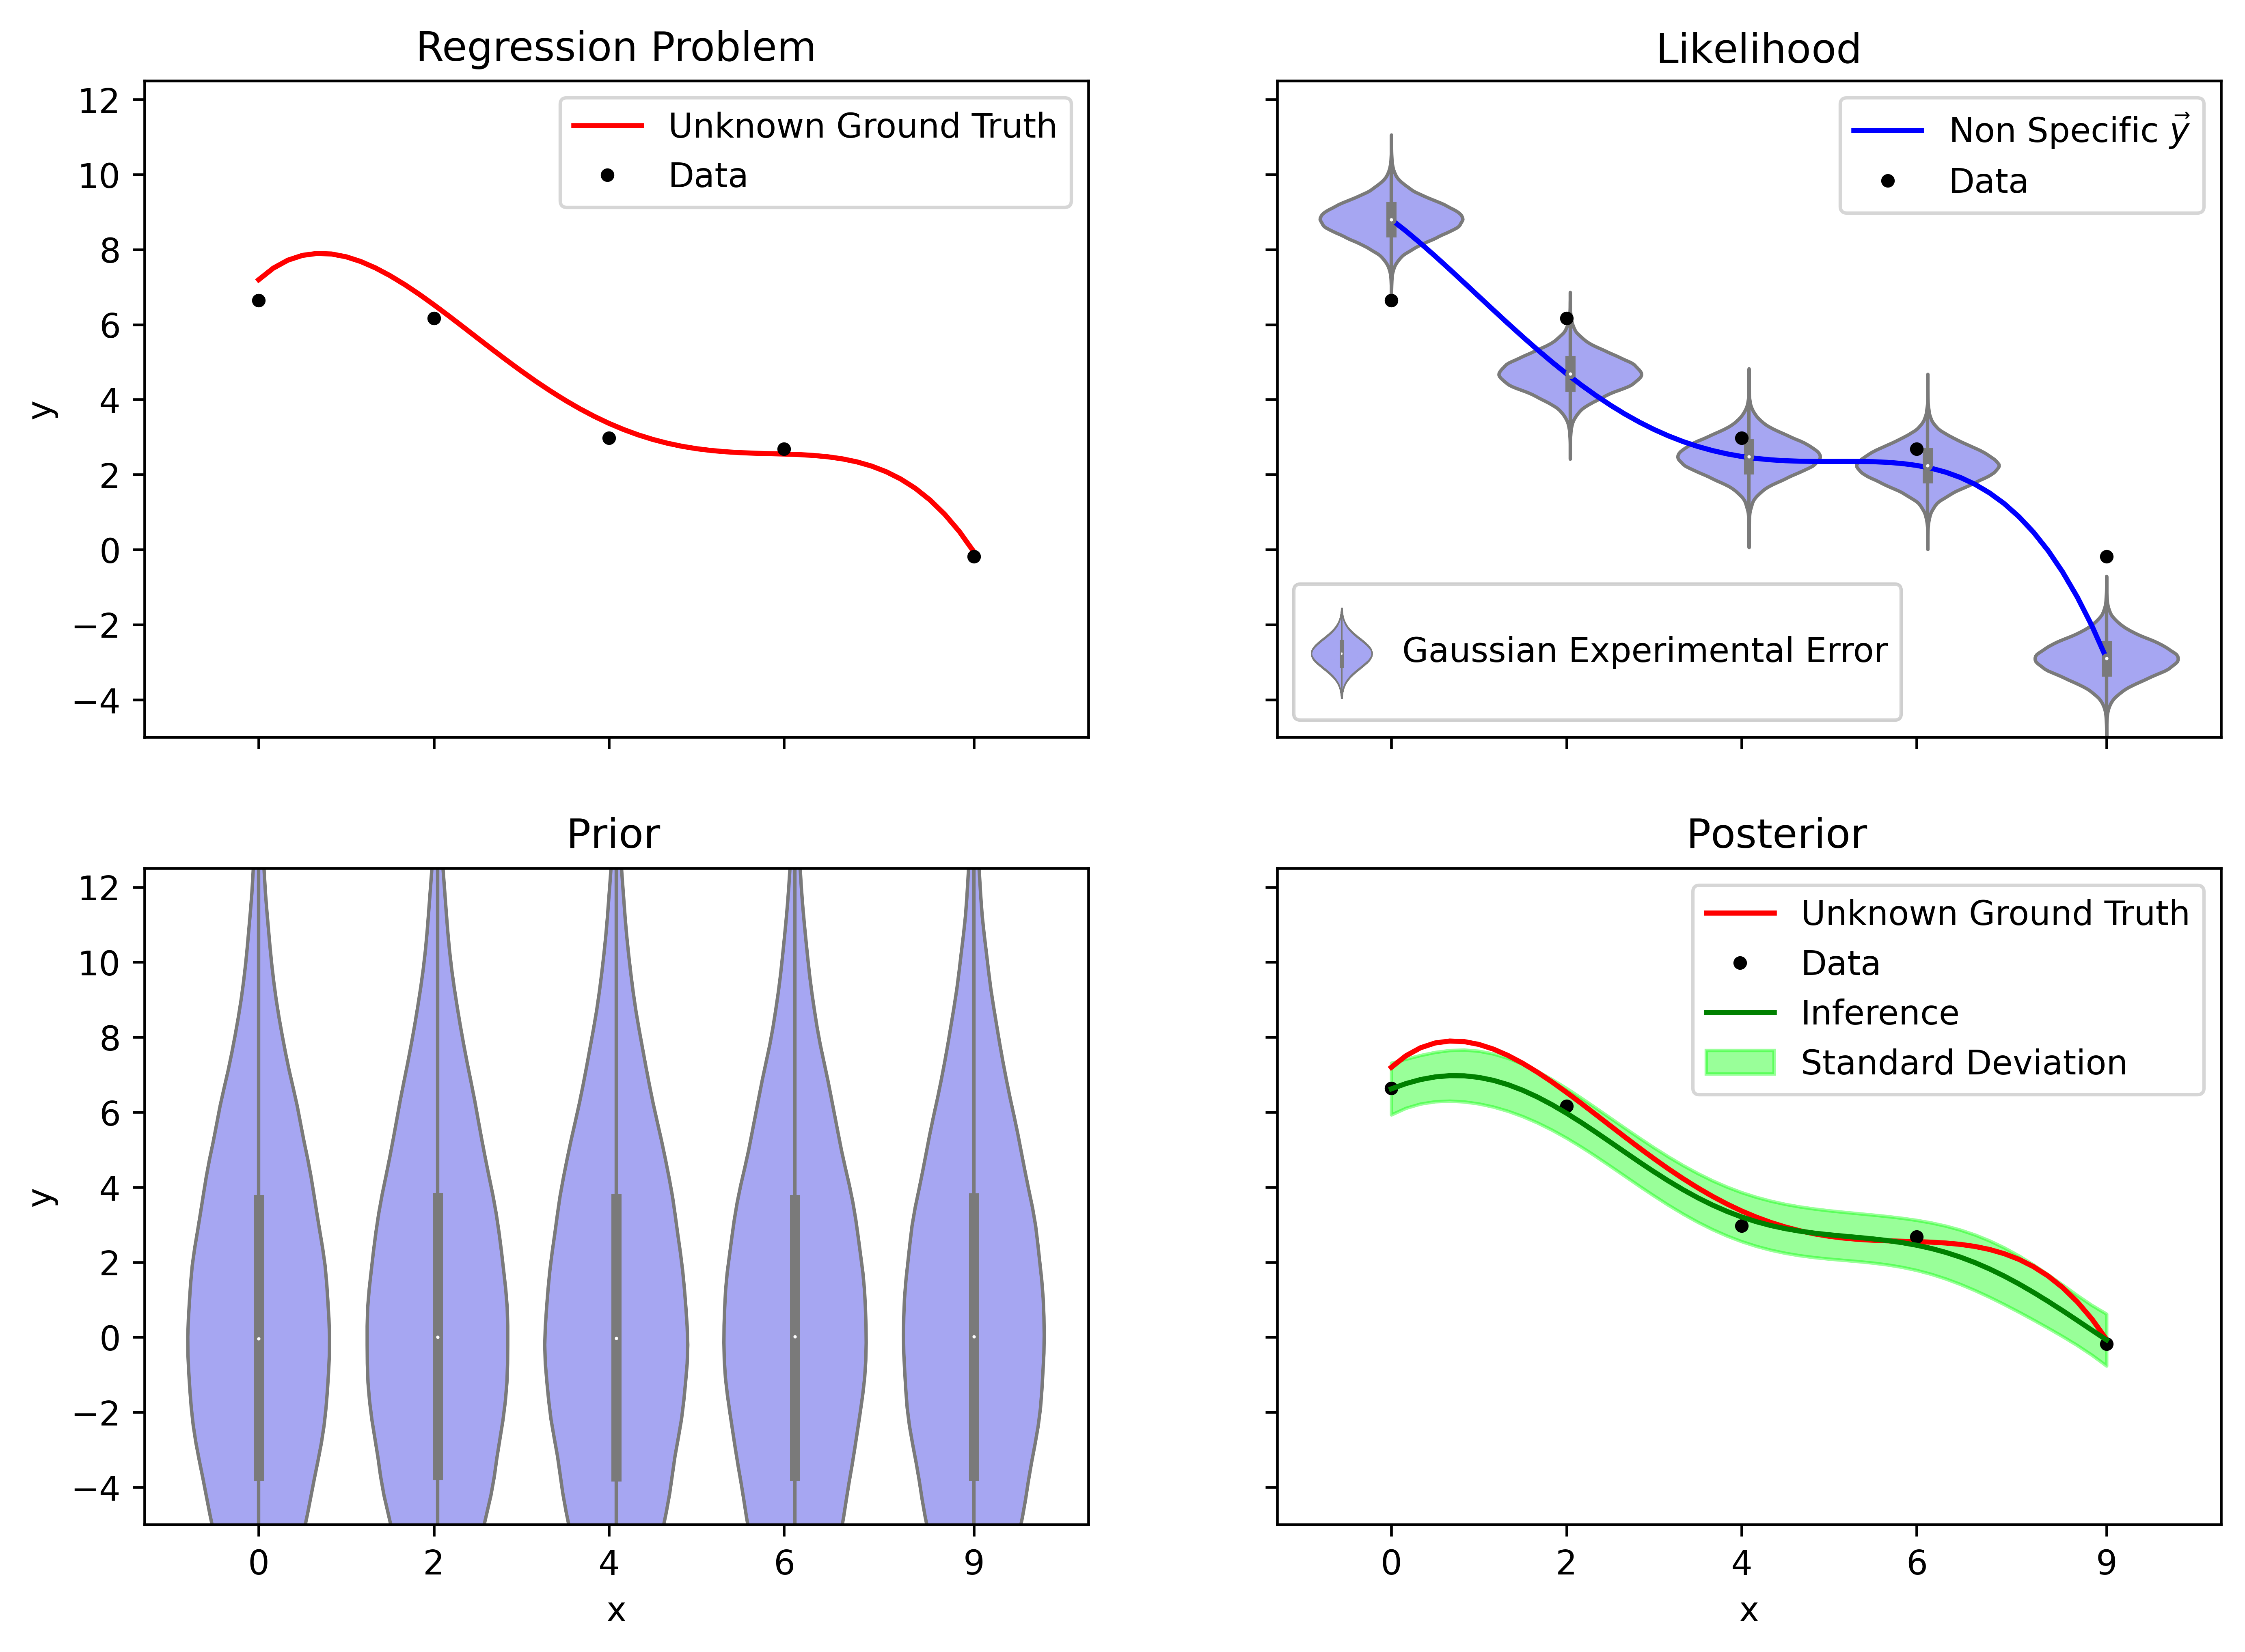
\includegraphics[width=13cm]{images/srpvis.png}
  \caption{A visualisation of the simple regression problem and the various distributions involved in the Bayesian inference solution.}
  \label{fig:srpvis}
\end{figure}

Figure \ref{fig:srpvis} shows the simple regression problem, it then tries to show the Gaussians that make up the likelihood and prior although it is not perfect. We assume the observations are independant giving the likelihood a diagonal covariance matrix. So the multiple Gaussians that make up the likelihood are not dependent on each other, thus representing them individually provides all the information in the likelihood. The prior has a more complex covariance matrix $K$, and figure \ref{fig:srpvis} does not have a complete representation of the priors form. Figure \ref{fig:srpvis} also shows the 101 gaussians that make up the posterior by plotting the regularly spaced $\vec{\mu}_{post}$ values in green with a green shadow showing the standard deviations of each gaussian that are found in the diagonal of $\Sigma_{post}$. The posterior mean vector and covariance matrix can be computed with the closed form expressions,

\begin{align}
\label{eq:mupost}
\vec{\mu}_{post} &= \vec{\mu}_{pr} + (K^{-1} + R^{\top} \Sigma_{li}^{-1} R)^{-1} R^{\top} \Sigma_{li}^{-1} (\vec{d} - R \vec{\mu}_{pr}),\\
\label{eq:covpost}
\Sigma_{post} &= \left(R^\top \Sigma_{li}^{-1} R + K^{-1}\right)^{-1},
\end{align}

\noindent which are derived in appendix \ref{append:dervcf}. The main steps include multiplying the functional forms of the prior and likelihood, ignoring all scaling factors, simplifying until they form a single unnormalised multivariate Gaussian and then comparing this with the posterior. The marginal likelihood can be expressed as,

\begin{equation}
\begin{aligned}
 P(\vec d|\vec\epsilon,\theta) &= \int P(\vec{d}|\vec{y},\vec\epsilon)P(\vec{y}|\theta)  \, d\vec y \\
 &= \frac{1}{(2\pi)^{\frac{m}{2}} \sqrt{|\Sigma_{li} + RKR^\top|}} \exp\left[ -\frac{1}{2} (\vec{d} - R\vec{\mu}_{pr})^{\top} (\Sigma_{li} + R K R^{\top})^{-1} (\vec{d} - R\vec{\mu}_{pr}) \right].
\end{aligned}
\end{equation}

\noindent The values of the marginal likelihood can become very large and troublesome to compute with standard 64-bit float precision. For this reason, the logarithm is computed. It is the convention when performing optimisation to define a loss function to be minimised, thus the negative log marginal likelihood is used. Scaling constants do not affect the minimum value and can be ignored. The negative log marginal likelihood used as a loss function for hyper-parameters is then,

\begin{equation}
loss(\vec \epsilon,\theta) = \ln(|\Sigma_{li}+RKR^\top|) +  (\vec{d} - R\vec{\mu}_{pr})^{\top} (\Sigma_{li} + R K R^{\top})^{-1} (\vec{d} - R\vec{\mu}_{pr}),
\end{equation}

\noindent the full derivation of this expression can be found in appendix \ref{append:dervml}.


\section{Interferometry and Polarimetry}

\begin{figure}[H]
  \centering
  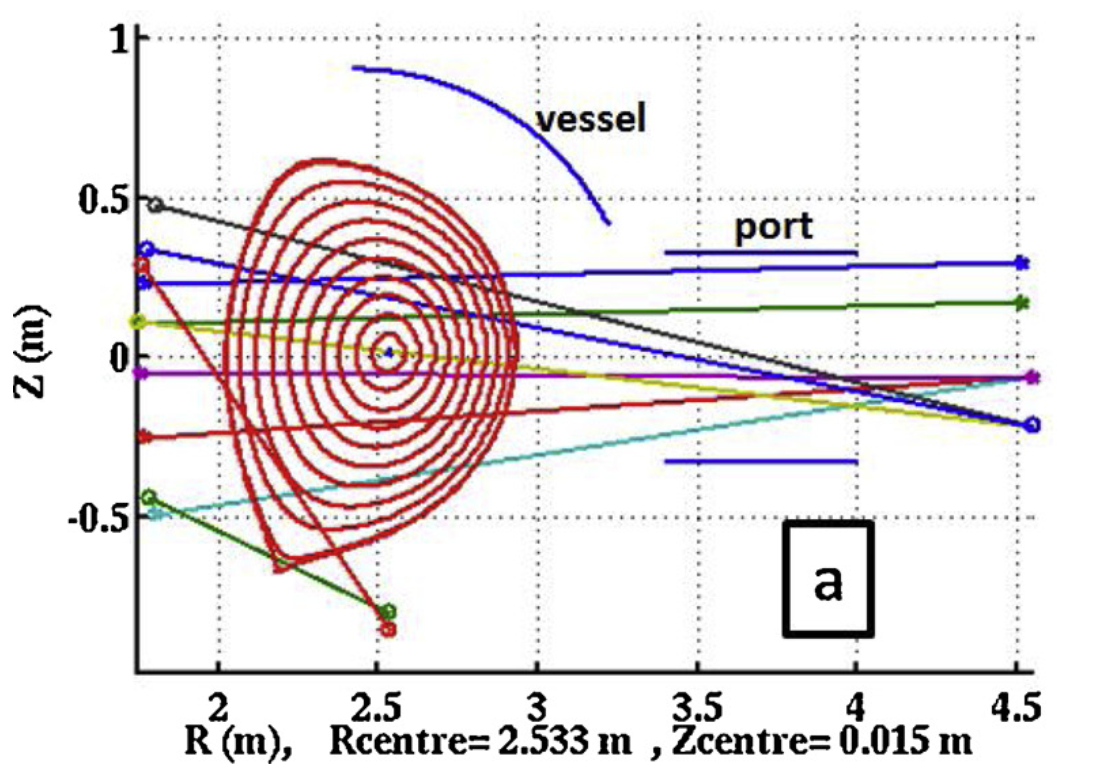
\includegraphics[width=10cm]{images/interfgeo.png}
  \caption{The geometry of interfero-polarimetry lasers at WEST \cite{westinterfero}.}
  \label{fig:interfgeo}
\end{figure}

Interferometry and Polarimetry are techniques that use the interference of electromagnetic waves to measure the properties of a medium. Interfero-polarimetry lasers within a tokamk penetrate the plasma at various angles. The geometry at \gls{west} is shown in figure \ref{fig:interfgeo}. Each laser is split into two beams: one that passes through the plasma and one that bypasses it. The two beams are then recombined and detected by a receiver. The phase difference between the two beams depends on the difference in the optical path length, which is affected by the electron density along the line of sight. Interferometry measures the phase difference; alowing one to calculate the line integrated electron density of the plasma $\int n_e \, dl$, 

\begin{equation} 
  \label{eq:int_phase}
  \Delta\phi = \frac{\lambda e^{2}}{4 \pi \epsilon_0 m_e c^2 } \int n_e \, dl \, \cite{princPlasDiag}.
\end{equation}

\noindent The laser wavelength $\lambda$, is combined with other common physical constants to ascertain the constant of proportionality. \gls{west} has stored the line integrated electron density as raw interferometry data in the \gls{imas} database. This is the data that will be used for this work. Although there is not enough information to completly and accuratly reconstruct the electron density profile a best guess given the data can be infered.

Polarimetry measures the Faraday rotation angle of the lasers. The linearly polarised lasers experience a rotation as the circularly polarised components travel through the plasma at different speeds. This is due to the small gyration of the electrons around the magnetic field. The Faraday rotation angle is proportional to the line integrated density of $n_e B_{||}$ along the line of sight of the lasers, 

\begin{equation}
  \label{eq:pol_farad}
  \theta_F = \frac{\lambda^2 e^3}{8 \pi^2 c^3 \epsilon_0 m_e^2} \int n_e B_{||} \, dl \, \cite{princPlasDiag},
\end{equation}

\noindent where $B_{||}$ is the magnetic field strength parallel to the line of sight. Polarimetry has information about electron density and this work could be extended to become a Bayesian integrated analysis which includes this information in the inference. Only interferometry information is used in this thesis. Polarimetry can be used in combination with interferometry to gain information about the poloidal magnetic field and this is why \gls{nice} uses it to determine the position of the magnetic flux surfaces.

\section{Bayesian Inference for Interferometry}\label{sec:InfForInterf}

To infer the electron density profile with interferometry, the previously defined regression process is altered. $\vec{y}$ becomes $\vec{n_e}$, the $\vec{0}$ prior mean can remain the same. The amplitude $\sigma$ and length-scale $l$ can be re-optimised by maximising the marginal likelihood. The data is now in a different space and thus is the likelihood. The response matrix $R$ must be created so that it will transform a profile $\vec{n_e}$ into what would be measured by an error free version of the \gls{west} interferometry system given $\vec{n_e}$ is the true profile. The result of $R \vec{n_e}$ is a vector the same length as the data $\vec{d}$ where each element corresponds to a different interferometry laser or channel. 

The response matrix computation can be summarised in a few steps. \Gls{nice} provides the magnetic flux at a set of grid points on the tokamak poloidal cross-section. It also provides the flux at a set of flux surfaces. The normalised radius $\rho$ of each flux surface is known. A simple 1D interpolation can be used to determine the normalised radius at each grid point. Then using $\vec{n_e}$ another 1D interpolation can be done to determine the electron density at each grid point. After the density at any point along a laser's line of sight $n_e(l_i)$, can be computed using triangular mesh interpolation. The density at the golden cross in figure \ref{fig:meshtriangle} can be computed as a weighted sum of the density at the three nearest grid points $\{g_1, g_2, g_3\}$ that form the golden triangle,

\begin{figure}
  \centering
  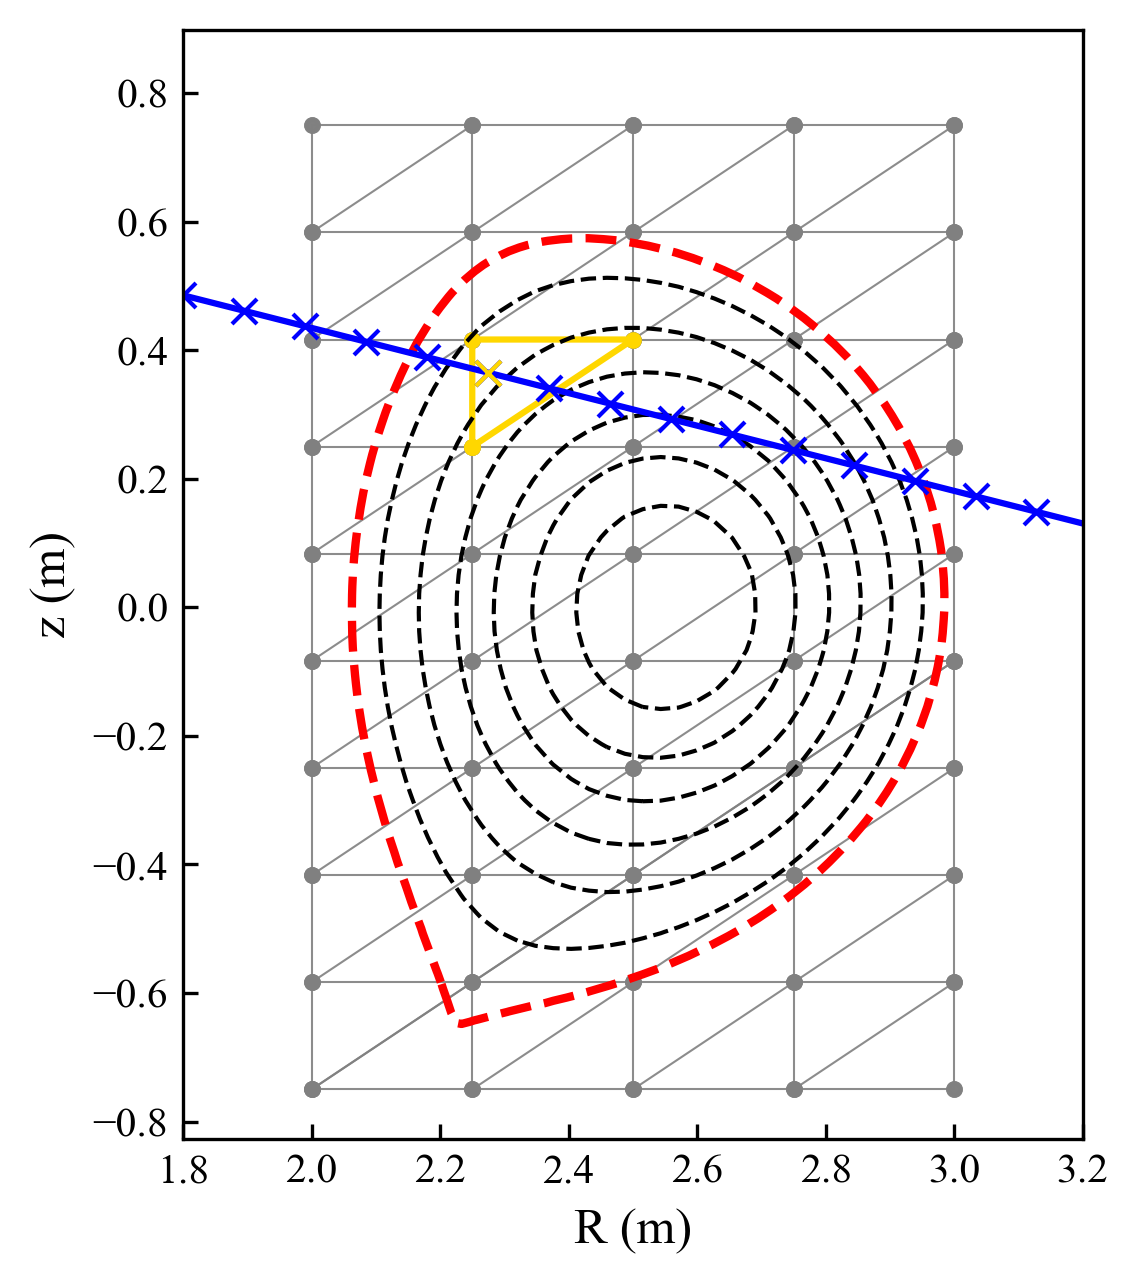
\includegraphics[width=10cm]{images/meshtriangle.png}
  \caption{An example mesh grid to aid visualisation of the triangular mesh grid interpolation used in the response matrix construction.}
  \label{fig:meshtriangle}
\end{figure}

\begin{equation}
  n_e(l_i) = \lambda_1 n_e(g_1) + \lambda_2 n_e(g_2) + \lambda_3 n_e(g_3),
\end{equation}

\noindent where $\lambda$ values can be computed using the $(R_1,z_1), (R_2,z_2), (R_3,z_3)$ coordinates of the 3 known density points and the point of interest $(R, z)$,

\begin{gather}
\lambda_1 = \frac{(z_2 - z_3)(R - R_3) + (R_3 - R_2)(z - z_3)}{(z_2 - z_3)(R_1 - R_3) + (R_3 - R_2)(z_1 - z_3)},\\
\lambda_2 = \frac{(z_3 - z_1)(R - R_3) + (R_1 - R_3)(z - z_3)}{(z_2 - z_3)(R_1 - R_3) + (R_3 - R_2)(z_1 - z_3)},\\
\lambda_3 = 1-\lambda_1-\lambda_2.
\end{gather}

\noindent These $\lambda$ values are known as the barycentric coordinates of the point of interest. The line integrated density can be approximated as a sum of electron densities at many points along the line of sight, $l_i$, times the width of their separation $\Delta l$,

\begin{equation}
  \int n_e \, dl \approx \sum_i n_e(l_i) \Delta l.
  \label{eq:neapprox}
\end{equation}

\noindent The contribution $w(g_i)$ of each grid point $g_i$ is a sum of all the mesh interpolation coefficiants $\lambda_j$ used on that point,

\begin{equation}
  \int n_e \, dl \approx \Delta l \sum_i w(g_i) n_e(g_i), \, w(g_i) = \sum_j \lambda_j.
\end{equation}

\noindent Each point can be associated with the nearest flux surface $f_i$ equally spaced in $\rho$. This way the contribution $w(f_i)$ of each flux surface is a sum of the contribution at each of its associated grid points $g_j$,

\begin{equation}
  \int n_e \, dl \approx \Delta l \sum_i w(f_i) n_e(f_i), \, f = \sum_j g_j.
  \label{eq:neapproxFS}
\end{equation}

\noindent All of these steps equate to a simple re-ordering of the original summation \ref{eq:neapprox} to extract the contribution of each flux surface on the final integrated density value. Equation \ref{eq:neapproxFS} can be computed using a vector product,

\begin{equation}
  \int n_e \, dl \approx \Delta l \vec{w}^{\top} \vec{n_e}.
\end{equation}

\noindent The contribution vector applies to one line of sight. The computation for all lines of sight can be performed by placing the $\Delta l \vec{w}$ vector for each line of sight as a row in the response matrix $R$. Thus, a vector of line integrated densities for the likelihood can be created,

\begin{equation}
  \vec{\mu_{li}} = R \vec{n_e}.
\end{equation}

\noindent This responce matrix $R$ can then be used in the closed form expressions \ref{eq:mupost} and \ref{eq:covpost}, to perfrom a 1D electron density profile inference.

Some further alterations to the inference method can be made to further increase reliability. These include altering the kernel and adding artificial observations to include prior knowledge. The kernel can be changed to a non-stationary kernel, 

\begin{equation}
  K_{ij} = k(\rho_i, \rho_j) = \sigma^2 \left( \frac{2l(\rho_i)l(\rho_j)}{l(\rho_i)^2 + l(\rho_j)^2} \right)^{1/2} \exp\left({\frac{(\rho_i - \rho_j)^2}{l(\rho_i)^2+l(\rho_j)^2}}\right),
\end{equation}

\noindent this allows the length scale to change as a function of $\rho$. The length scale controls smoothness, model complexity and curvature. If these are free to change for different regions of the plasma then there is a greater range of possibilities for the final inference. Chilenski used a hyperbolic tangent function,

\begin{equation}
  l(\rho) = \frac{l_{core} + l_{edge}}{2} + \frac{l_{core} - l_{edge}}{2} \tanh\left(\frac{\rho-\rho_{step\,center}}{\rho_{step\,width}}\right) \, \cite{chilenski}, 
  \label{eq:smoothstep}
\end{equation}

\noindent to form a smooth step down from a high length scale at the core to low at the edge, see figure \ref{fig:smoothstep}. The extra freedom at the edge allows the inference to accommodate for a large sudden drop in electron density, which is a common feature for H-mode plasmas. H-mode plasmas are known to have a longer confinement time and thus better fusion performance. \gls{west} does not operate in H-mode, although this method is tested with synthetic data from a simple H-mode simulation.

\begin{figure}[H]
  \centering
  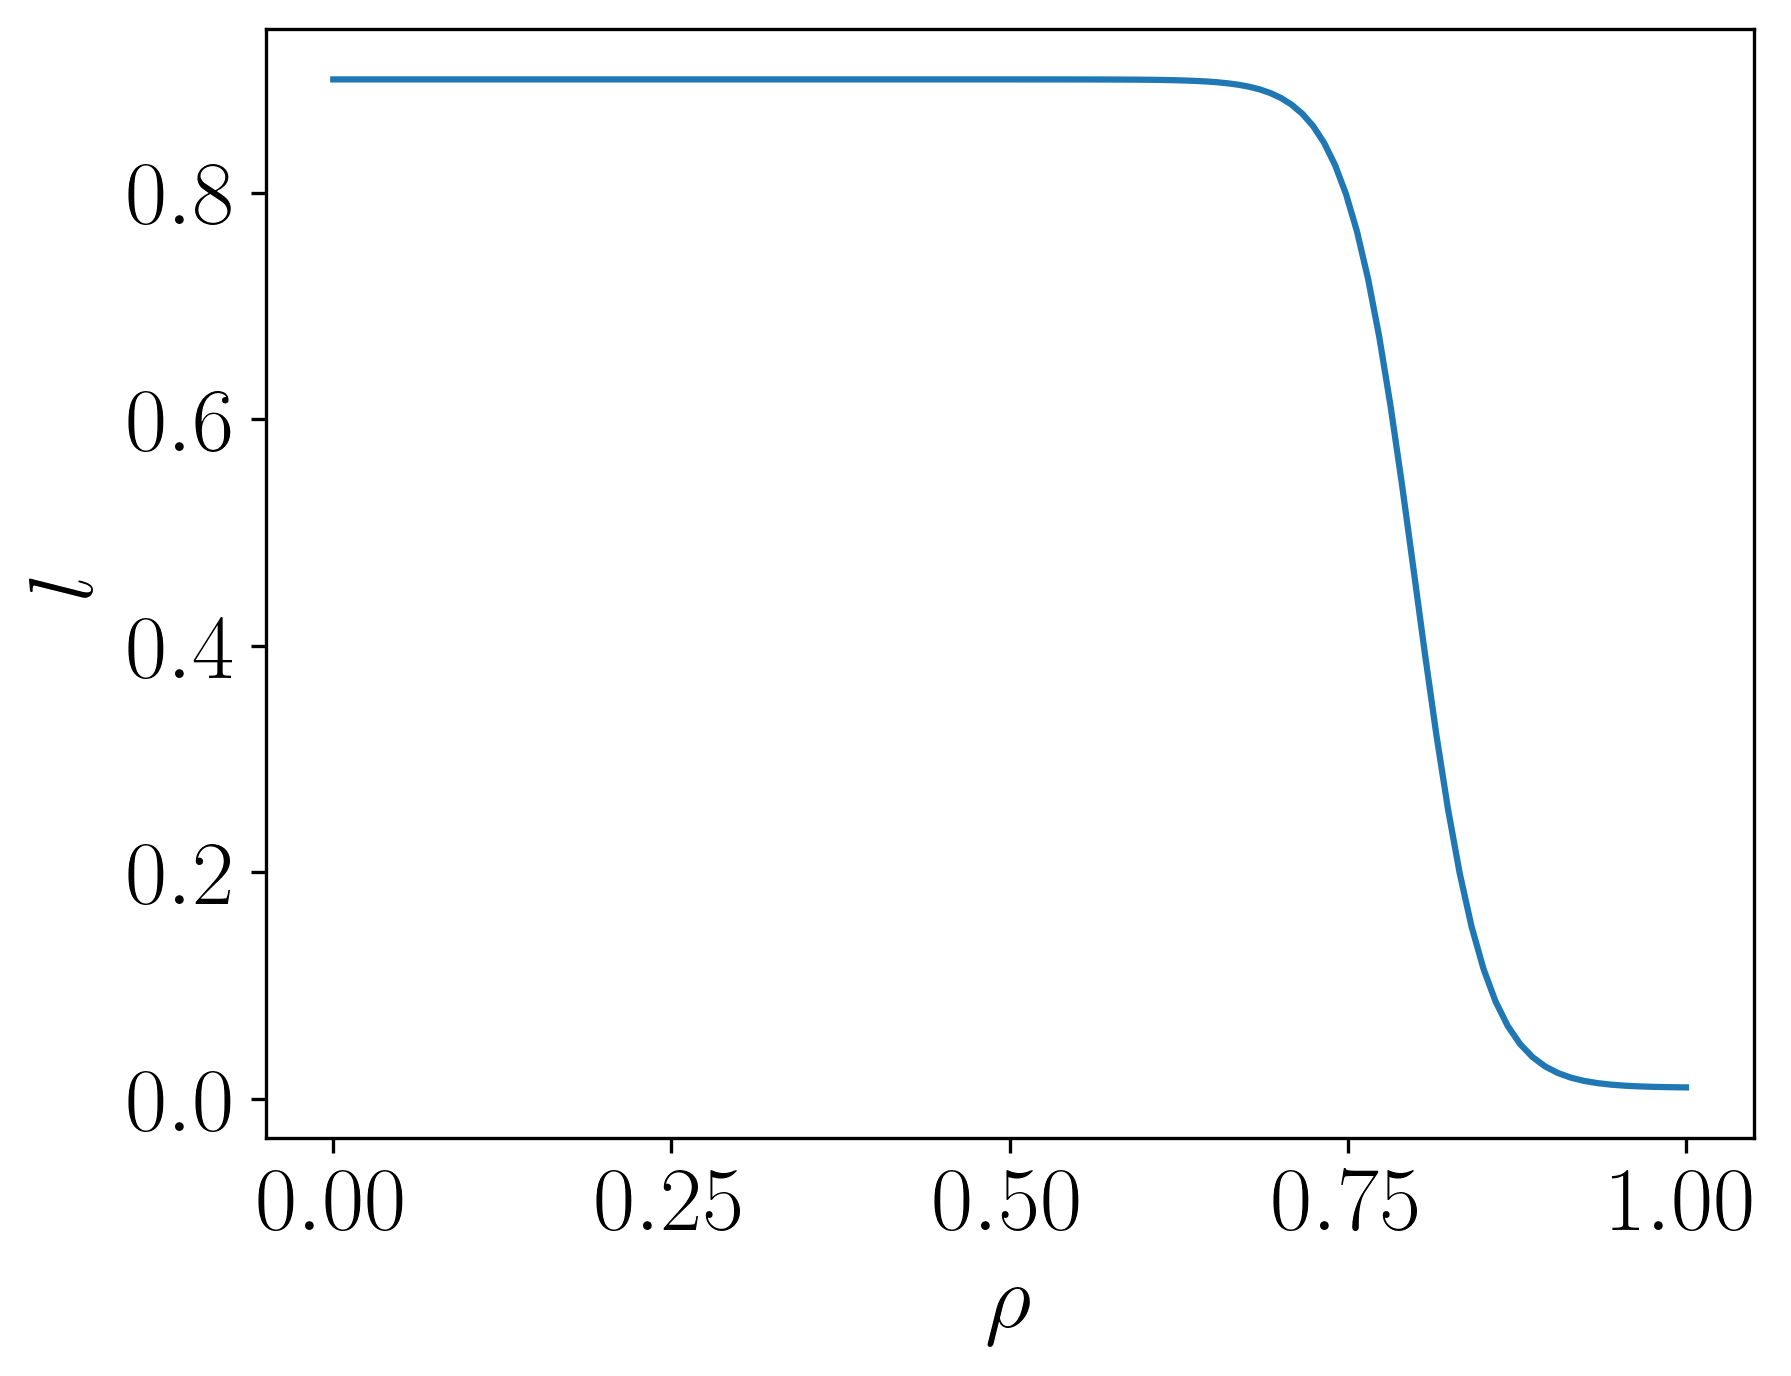
\includegraphics[width=10cm]{images/smoothstep.png}
  \caption{Hyperbolic tangent smooth step function for length scale, equation \ref{eq:smoothstep}. Used to capture the drop at the edge of H-mode plasmas \cite{chilenski}.}
  \label{fig:smoothstep}
\end{figure}

% Explain the cubic spline length scale here if it is done in the results 

Traditionally prior information should be included in the prior distribution. However, in practice precision errors can make this difficult. The closed form expressions for $\vec{\mu}_{post}$ and $\Sigma_{post}$ involve inversions of both the likelihood and prior covariance matracies, although the likelihood covariance matrix $\Sigma_{li}$ is diagonal and so is certinly positive definate and inversion does not suffer from precision errors. This is not true for the priors covariance matrix $K$, it is difficult to define a prior covariance matrix that includes all the prior information, remains non positive definate and does not suffer from precision errors. For these reasons it is often more convenient to place prior information into the likelihood in the form of artificial observations. This method was also adopted by Chilenski \cite{chilenski}. The density is known to be close to 0 at the plasma boundary, ($\rho=1$). It is also known that the density profile is smooth and symmetric meaning the gradient of the profile on the magnetic axis must be close to 0. This information can be included in the data, $\vec{d}$, with an artificial experimental error determining the strength of the information included in $\vec{\epsilon}$. Other parts of the method need to be altered to accommodate the new information. The vector to be infered $\vec{a}$ is not only $\vec{n_e}$ but also includes $n_e(\rho=1)$ and $n_e'(\rho=0)$ concatonated onto the end. This allows the response matrix alteration to be simple,

\begin{equation}
  R^{alt} = 
\begin{bmatrix}
 R_{m\times n} &   O_{m\times2} \\
 O_{2\times n} &   I_{2\times 2} \\
\end{bmatrix}
=
\begin{bmatrix}
 &       &    & 0         & 0\\
  &   R_{m\times n}    &    &  \vdots  & \vdots\\
  &       &    & 0        & 0\\
0 & \cdots & 0  & 1        & 0 \\
0 & \cdots & 0  & 0        & 1
\end{bmatrix},
  \label{eq:Ralt}
\end{equation}

\noindent where $n$ is the number of unknown electron density values in $\vec n_e$ and $m$ is the number of interferometry lasers. The prior covariance matrix must also be altered. The covariance between a gradient and non-gradient data point is simply the differential of the covariance over the gradient data point. For two gradient data points, it is a differential over each point.

\begin{equation}
  K'_{ij} = k'(\rho_i, \rho_j) = \frac{\partial k'(\rho'_i, \rho_j)}{\partial \rho'_i} \, \cite{chilenski},
\end{equation}

\begin{equation}
  K''_{ij} = k''(\rho'_i, \rho'_j) = \frac{\partial k''(\rho'_i, \rho'_j)}{\partial \rho'_i \partial \rho'_j} \, \cite{chilenski}.
\end{equation}

\noindent In this notation $\rho'$ indicates the position of a gradient data point. The alternate kernel is then,

\begin{equation}
  K^{alt} = 
    \begin{matrix}
      K & K'\\
      K'^{\top} & K''
    \end{matrix}.  
\end{equation}

The necessary adaptations to our defined Bayesian regression method to accomodate interferometry data have been described. For reference, the various final distributions and expressions after the adaptations are fully shown in appendix \ref{append:distexpres}.

\section{Chapter Summary}

The electron density profile is important as it plays a key role in determining the energy confinement time and informing real time control systems. With the assumption of magnetic flux surfaces, one can express it as a 1D profile. \gls{nice} is an equilibrium reconstruction code that also infers the electron density profile that can be used as a comparison in this thesis. Bayesian inference with multivariate gaussians describing the various distributions can be applied to interferometry data to infer the electron density profile. A non-stationary kernel can be used to allow the inference to have a model complexity that varies with $\rho$. Hyperparameters can be tuned by minimising the negative log marginal likelihood. Prior information can be easily included in the likelihood with artificial observations. In the results section, these methods will be deployed on synthetic data. The inference performance can be determined by how closely it fits the ground truth profile. They will also be deployed on real \gls{west} data and the results will be compared to that obtained by \gls{nice}.
% \begin{figure}
%   \centering
%   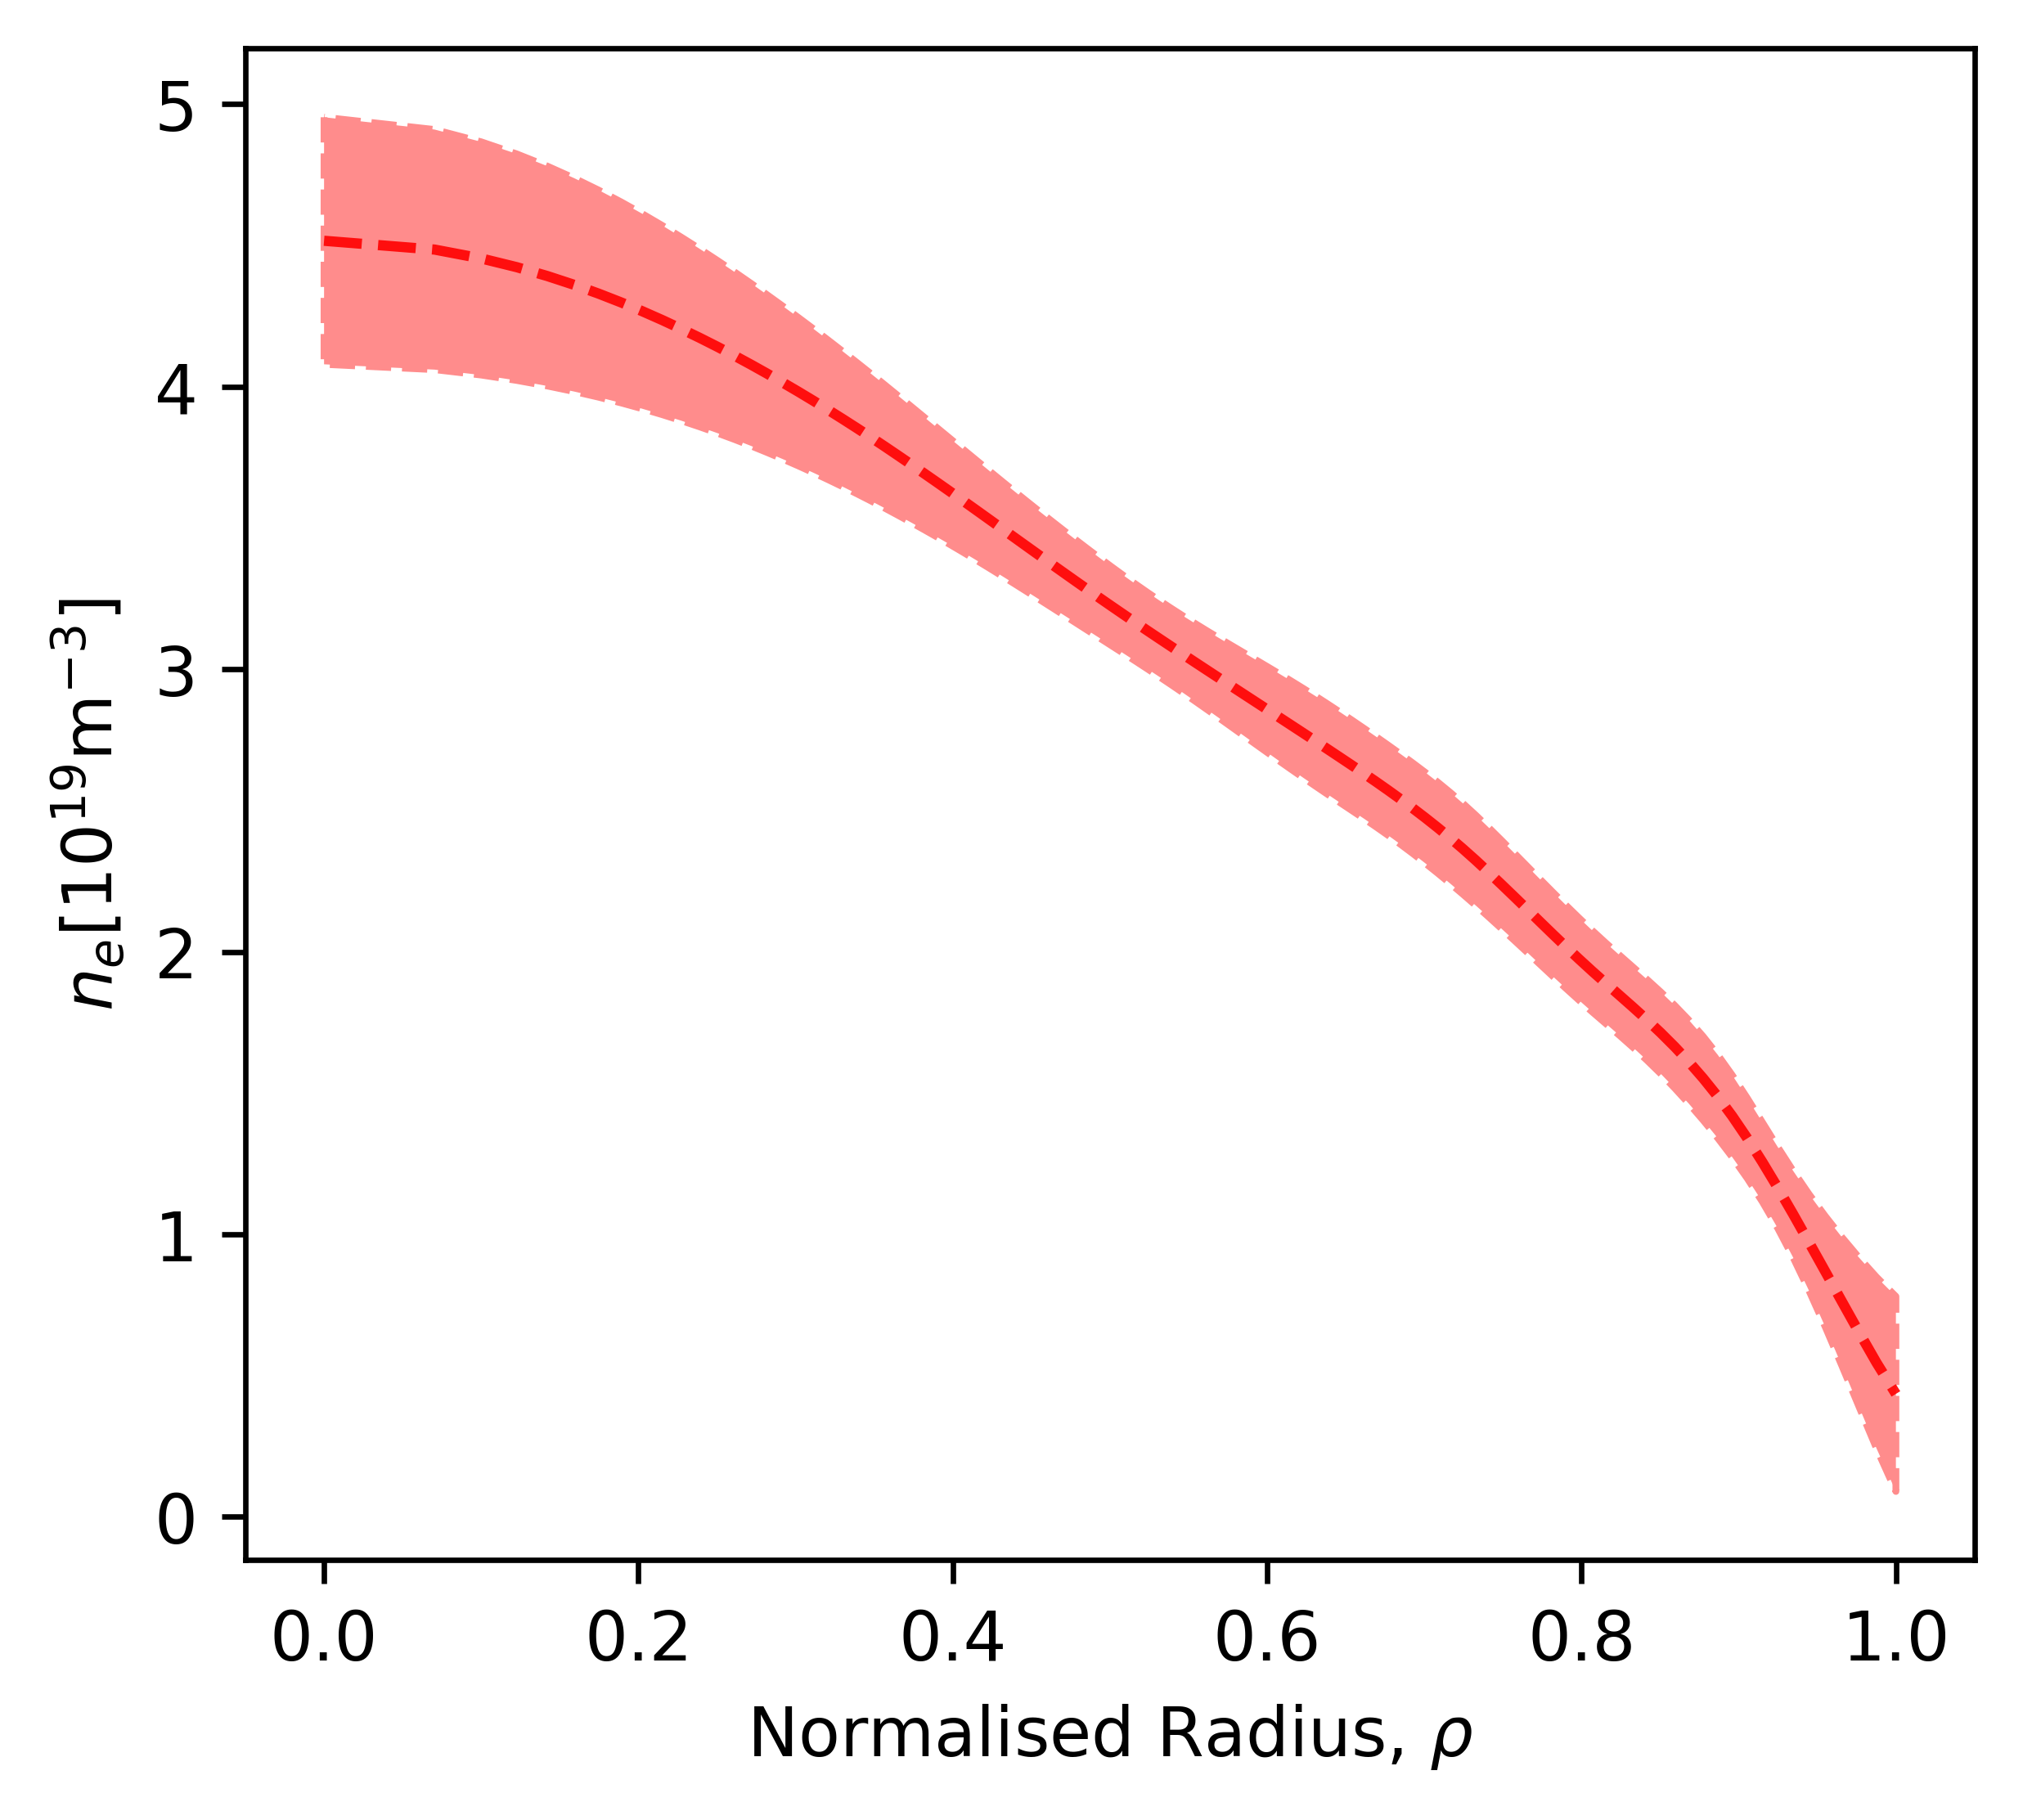
\includegraphics[width=\columnwidth]{images/niceExample.png}
%   \hskip 1mm
%   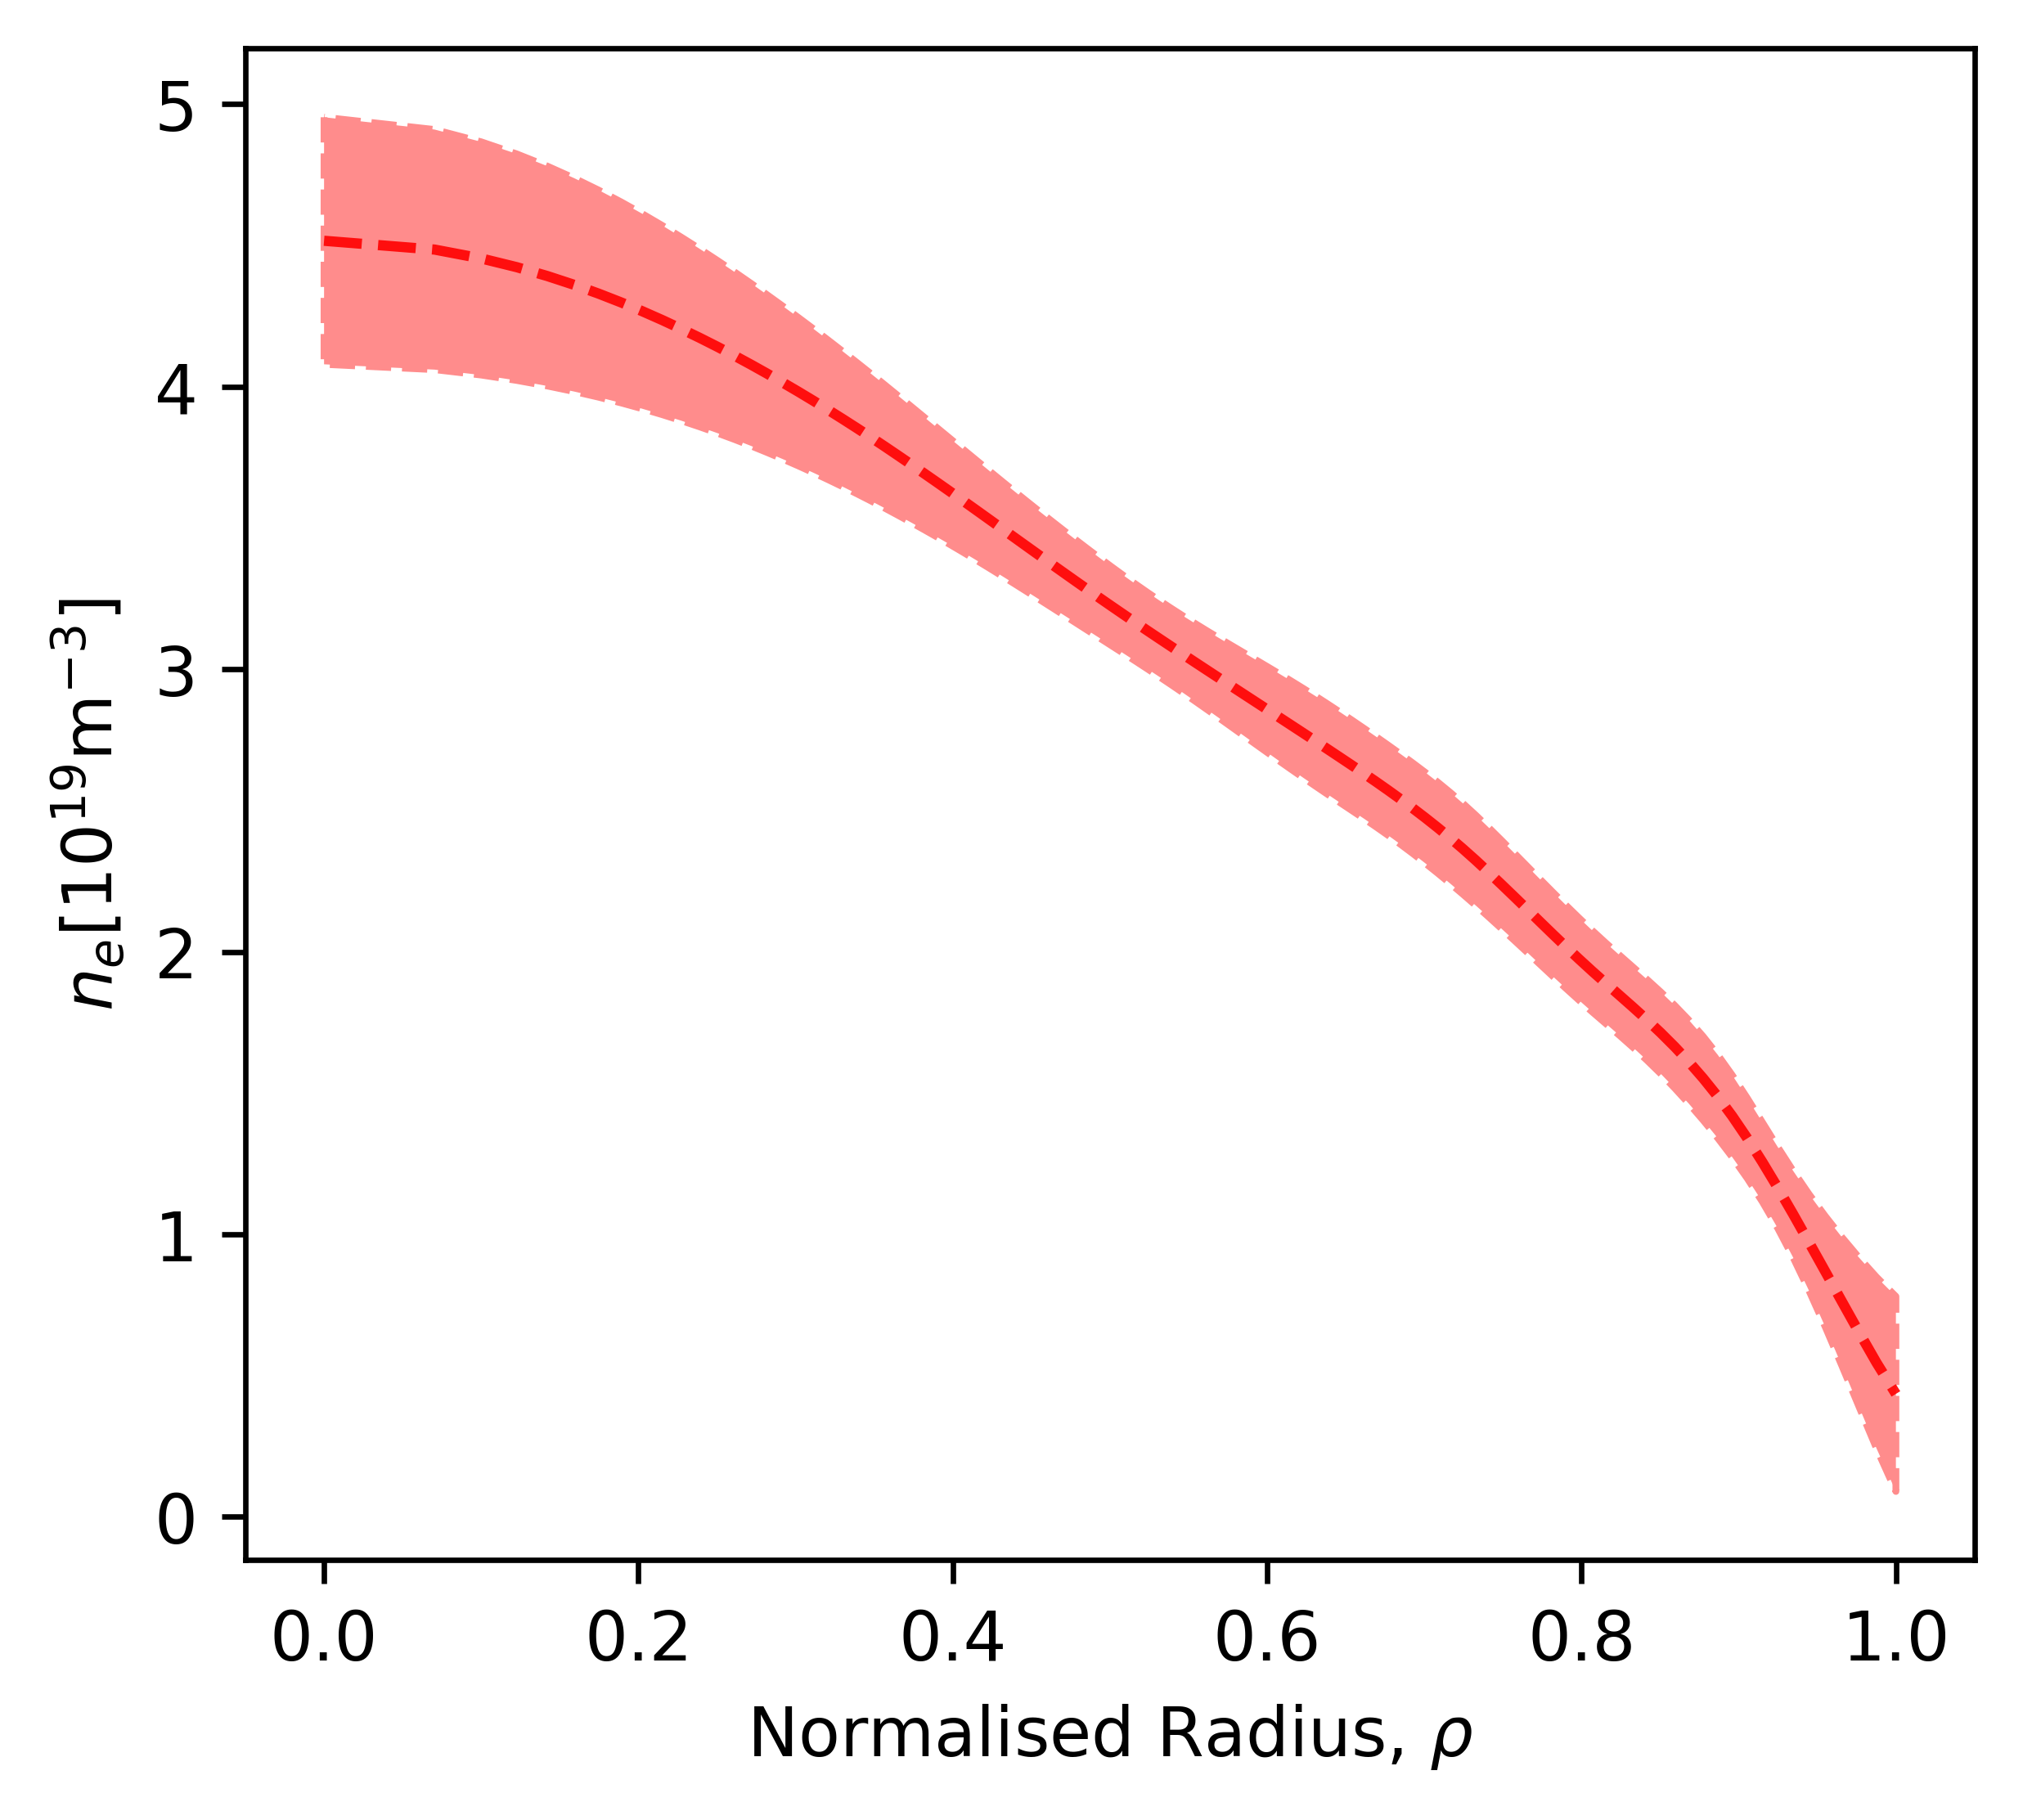
\includegraphics[width=\columnwidth]{images/niceExample.png}
%   \hskip 1mm
%   \vspace{-1cm}
%   \caption{Predictions on completely sampled space.}
%   \label{fig:flowe_grid}
% \end{figure}

% \label{sec:intpol}
% \section{Interfero-polarimetry}


% \begin{itemize}
%     \item Some basic background theory of a tokamak as a fusion device. Including the schematics of the magnetics and different systems present. Including the magnetic flux surfaces and what they are, assumptions made. What is $\rho$? Also highlights a little why the plasma density profile is important. 
%     \item Explain the theory of how NICE did their inference to some degree. ***
%     \item Bayes' theorem for inference problems, each distribution involved and why the marginal likelihood is useful. ***
%     \item Explian how a multivariate gaussian can model a curve. ***
%     \item Explain Gaussian Process Regression for a generic line fitting problem, including the various distributions constructed and how they are used in the closed form expressions. A little on marginal liklyhood again for parameter optimisation. Mention briefly the alterations to this algorithm that will be made to allow it to be used for interferometry including the response function change, and virtual observations.
%     \item Explain Interferometry and a little on polarimetry, show west laser geometry
%     \item Explain the magnetic flux surfaces again a little and how this allows us to make the electron density profile 1D again.
%     \item Explain the forward model and how it is computed with the response matrix.
%     \item Explain how the prior edge and core information can be added and the complications of inserting it into the prior.
%     \item Explain why a non-stationary kernel (smooth step) might be beneficial 
%     \item summarise the chapter and explain how it ties into the methodology
% \end{itemize}